\documentclass[10pt,letterpaper,final]{article}
\usepackage[utf8]{inputenc}
\usepackage{amsmath}
\usepackage{amsfonts}
\usepackage{amssymb}
\usepackage{graphicx}
\usepackage[left=2cm,right=2cm,top=2cm,bottom=2cm]{geometry}
\usepackage{fullpage}
\author{Jun Ye Yu}
\title{Distributed particle filter for bearing-only tracking}
\begin{document}
\maketitle

\section{Introduction}
In this report we present four distributed particle filters for single-target bearing-only tracking. The first filter factorizes the log-likelihood function so that the joint log-likelihood function can be characterized using six constraint sufficient statistics. The second filter uses likelihood consensus to approximate the measurement function. The third filter constructs a graph over all particles and the Eigenvectors of the resulting Laplacian matrix are used to encode the particle log-likelihood. Finally, the fourth filter groups all particles into clusters and computes the cluster joint likelihood. The individual particle weights are recovered via convex minimization. For the remainder of the report, we refer to the four particle filters as \textbf{CSSpf}, \textbf{LCpf}, \textbf{LApf} and \textbf{Clusterpf}. We also include the centralized \textit{bootstrap particle filter} (\textbf{BSpf}) as baseline. 

The remainder of the report is organized as follows. Sec.~\ref{sec:problem} defines the tracking problem. Sec.~\ref{sec:pf} presents the particle filters. Sec.~\ref{} compares the filters' performance and Sec.~\ref{}

\section{Problem statement}
\label{sec:problem}
A network of $S$ sensors collaboratively track a single target over time. The sensors have fixed position $[x_s, y_s], s=1...S$. The target state at time $k$ is modeled as $X(k) = [x_t(k),y_t(k), \dot{x}_t(k), \dot{y}_t(k)]$ where $x_t(k)$, $y_t(k)$ are the target position and $\dot{x}_t(k)$, $\dot{y}_t(k)$ are its velocity. 

At time $k$, the target transitions to new state $X(k)$ with probability $f(X(k)|X(k-1))$ which depends on the target dynamic model. Each sensor $s$ also receives a measurement $z_s(k)$ with likelihood $f(z_s(k)|H_s(X(k))$ where $H_s(\cdot)$ is the (possibly sensor-dependent) measurement function. 

\section{Distributed particle filters for bearing-only tracking}
\label{sec:pf}
In Bayes' filter, we recursively estimate the posterior target density $f(X(k)|Z(1),...Z(k))$ where $Z(k) = \{ z_1(k)...z_S(k)\}$. In a particle filter, we model the target density using a set of $N$ particles with normalized weights $\{X_i(k), w_i(k)\}_{i=1}^N$. Therefore, the objective is to recursively estimate the posterior particle weights. This in turn requires the computation of joint log-likelihood:
\begin{equation}
\log(f(z_1(k),...z_S(k)|X_i(k)))=\sum_{s=1}^S\log\left(f(z_s(k)|X_i(k))\right)
\label{eqn:joint_log_lh}
\end{equation}
where we assume that measurements from different sensors are conditionally independent given the target state. 

We assume that the sensors receive bearing measurement corrupted by additive zero-mean Gaussian noise, and have the following measurement model:

\begin{equation}
H_s(X)= \arctan2 \left( \frac{x_t-x_s}{y_t-y_s} \right) + \eta_s
\end{equation}
where $\eta_s \sim \mathcal{N}(0, \sigma_s)$ is the measurement noise. 

The joint log-likelihood is thus
\begin{align}
\log(f(z_1,..., z_S|X) &\propto \sum_{s=1}^S \frac{-(z_s-H_s(X))^2}{2\sigma_s^2} \nonumber \\ 
&= \sum_{s=1}^S \frac{-(z_s)^2-H_s(X)^2+2z_sH_s(X)}{2\sigma_s^2}
\label{eqn:log_lh_normal}
\end{align}

For the remainder of this section, we present four distributed particle filters which differ in how they compute the joint log-likelihood. We omit time step indice $k$ where there is no ambiguity. 

\subsection{Constraint sufficient statistics particle filter}
In the CSSpf, the likelihood function can be approximated as follows:
\begin{equation}
\log(f(z_s|X) \approx \sum_{j=1}^6 G_{s,j}F_j(X)
\end{equation}
where the functions $F_j(X)$ depend only on $X$ and are known to all sensors. The sufficient statistics $G_{s,j}$ depend only on local information from sensor $s$. In other words, we approximate the log-likelihood function by the combination of six basis functions $F_j(X)$ with corresponding coefficients $G_{s,j}$. We omit the detailed expressions for $G_{s,j}$ and $F_j(X)$. 

This approximation leads to the following log-likelihood function
\begin{equation}
\log(f(z_1,..., z_S|X) \approx \sum_{j=1}^6 F_j(X) \left(\sum_{s=1}^S G_{s,j}\right)
\label{eqn:llh_css}
\end{equation}
where the summation terms $\left(\sum_{s=1}^S G_{s,j}\right)$ can be interpreted as the global sufficient statistics. 

The six global sufficient statistics can be computed in a distributed manner by running six consensus algorithms in parallel. 

\subsection{Likelihood consensus particle filter}
In LCpf, we approximate the measurement function as follows:
\begin{equation}
\hat{H}_s(X) = \sum_{j=1}^J \alpha_{s,j} \beta_j(X)
\label{eqn:Hx_LC}
\end{equation}
where $\beta_j(X)$ is the $j^{th}$ sensor-independent basis function and $\alpha_{s,j}$ is the corresponding coefficient that encompasses all the information of sensor $s$. 

Plugging Eq.~\eqref{eqn:Hx_LC} into Eq.~\eqref{eqn:log_lh_normal} yields
\begin{align}
\log(f(z_1,...z_S|X)) &\propto -\sum_{s=1}^S \frac{(z_s)^2}{2\sigma_s^2} -\sum_{s=1}^S \frac{\left( \sum_{j=1}^J \alpha_{s,j} \beta_j(X)\right)^2}{2\sigma_s^2} + \sum_{s=1}^S \frac{z_s\sum_{j=1}^J \alpha_{s,j} \beta_j(X)}{\sigma_s^2} \nonumber \\
&= -\frac{\sum_{s=1}^s(z_s)^2}{2\sigma_s^2} - \sum_{j=1}^J\sum_{l=1}^L\frac{\sum_{s=1}^s \alpha_{s,j}\alpha_{s,l} \beta_j(X)\beta_l(X)}{2\sigma_s^2}+ \sum_{j=1}^J\frac{\sum_{s=1}^S z_s \alpha_{s,j} \beta_j(X)}{\sigma_s^2} \nonumber \\
&= -\frac{\sum_{s=1}^S(z_s)^2}{2\sigma_s^2} - \sum_{m=1}^MB_{m}(X)\frac{\sum_{s=1}^S A_{s,m} }{2\sigma_s^2}+ \sum_{j=1}^J\beta_j(X)\frac{\sum_{s=1}^S z_s \alpha_{s,j} }{\sigma_s^2} 
\label{eqn:joint_log_lh_LC}
\end{align}
where, for the last equality, we employ a suitable mapping $m\rightarrow (j,l)$, $M=J*L$, $B_m(X)=\beta_j(X)\beta_l(X)$ and $A_{s,m} = \alpha_{s,j}\alpha_{s,l}$. 

Eq.~\eqref{eqn:joint_log_lh_LC} suggests that the joint log-likelihood can be constructed using consensus algorithms to compute the global sufficient statistics $\sum_{s=1}^S A_{s,m}$ and $\sum_{s=1}^S z_s\alpha_{s,j}$. The first term in Eq.~\eqref{eqn:joint_log_lh_LC} can be ignored since it is constant and independent of $X$. 

We now describe how to compute the coefficients $\alpha_{s,j}$ using the least-square approach. Given the $N$ particles $X_i$, we construct the matrix $\Phi$ as follows:
\begin{equation}
\Phi=\left(
\begin{array}{ccc}
\beta_1(X_1) & ... & \beta_J(X_1) \\
... & ... & ... \\
\beta_1(X_N) & ... & \beta_J(X_N)
\end{array}
\right)
\label{eqn:beta_matrix}
\end{equation}

For each sensor $s$, we also construct the following column vector
\begin{equation}
\Lambda_s = [ H_s(X_1), ... H_s(X_N)  ]^T
\label{eqn:lambda_vector}
\end{equation}
where $T$ denotes the transpose operation. 

The coefficients can be estimated as follows:
\begin{equation}
\alpha_s = [\alpha_{s,1},...\alpha_{s,J}]^T = (\Phi^T\Phi)^{-1}\Phi^T\Lambda_s
\end{equation}

\subsection{Laplacian approximation particle filter}
In LApf, we construct a K-nearest-neighbor graph using each particle $X_i$ as a vertex. The Laplacian matrix of the graph are used to construct a transformation that allows particle log-likelihoods to be represented using a minimal number of coefficients. 

Let $L$ denote the Laplacian matrix of the K-nearest-neighbor graph with eigenvalue decomposition $L=F^T\Lambda F$. We retain only the $m \leq N$  eigenvectors corresponding to the $m$ smallest eigenvalues and denote the resulting $N\times m$ matrix $F_m$. 

Let $\gamma_s = [\log (f(z_s|X_1), ... \log (f(z_s|x_N))]^T$ denote the column vector containing the log-likelihoods of all $N$ particles at sensor $s$. We compute the local coefficients at sensor $s$ as follows:
\begin{equation}
\alpha_s = F_m^T\gamma_s
\end{equation}

The global coefficients are the summation of local coefficients across all $S$ sensors: $\alpha = \sum_s \alpha_s$. 

The approximate joint log-likelihood can be computed as follows:
\begin{equation}
\hat{\gamma} = F_m\alpha
\end{equation}

\subsection{Clustering particle filter}
In Clusterpf, the particles are grouped into $C$ clusters based on their position. The log-likelihood of each cluster is equal to the aggregate log-likelihood of its constituent particles. Consensus algorithms are used to compute the global 
cluster log-likelihood. 

\section{Performance evaluation}
\subsection{Simulation setup}
We compare the performance of likelihood consensus filter against that of a centralized bootstrap filter and a second distributed filter based on constraint sufficient statistics. 

We construct a network of 9 sensors in a $3\times 3$ grid. The target starts near the center sensor and travels in clockwise direction over 50 time steps. The sensors remain static over time. The target position is measured in longitude and latitude and the target velocity is measured in km/time step. Fig.~\ref{fig:track} shows a sample target trajectory and sensor positions. 

The simulated target randomly switches between two different motion models: constant velocity with probability $P_{cv}$ and coordinated clockwise turn with probability $1-P_{cv}$. 

All sensors receive bearing measurements (in radians) from the target:
\begin{equation}
z_s(X) = \arctan2 \left( \frac{\sin(x_t-x_s)\cos(y_t)}{\cos(y_s)\sin(y_t)-\sin(y_s)\cos(y_t)\cos(x_t-x^s)}  \right)
\label{eqn:bearing}
\end{equation}

We also inject additive white Gaussian motion and measurement noise with covariance $Q$ and $R$ respectively.
\begin{align}
Q &= \sigma_a^2
\left[
\begin{array}{cccc}
\frac{T^3}{3} & 0 \frac{T^2}{2} & 0 \\
0 & \frac{T^3}{3} & 0 \frac{T^2}{2} \\
\frac{T^2}{2} & 0 T & 0 \\
0 & \frac{T^2}{2} & 0 T \\
\end{array}
\right]\\
R &= \sigma_{\theta}^2
\end{align}
where $\sigma_a=10^-4$, $T=1$ and $\sigma_{\theta}=0.0873\text{ rad} = 5 \text{ degree}$.

\begin{figure}
\centering
\includegraphics[width=0.75\textwidth]{Figures/Track}
\caption{Target trajectory (blue curve) and sensor positions (red diamond)}
\label{fig:track}
\end{figure}

\subsection{Algorithm setup}
All particle filters use a total of $N$ particles. At time step 1, we generate the initial particles using the true target state: $X_i(1) \sim \mathcal{N}(X_i(1), X(1), R_{\text{initial}})$ with $R_{\text{initial}}=\text{diag}([10e^{-4},10e^{-4},10e^{-5},10e^{-5}])$. 

All three particle filters use the same dynamic model, and
they only differ in the likelihood evaluation. We further assume that the random number generators are synchronized across the sensors. 

For the CSSPF and LCPF, we compute the global sufficient statistics exactly (i.e., without gossiping or consensus) so that all difference in tracking performance comes from likelihood computation. 

For LCPF, we consider two different sets of basis functions. Consider a set of points in the tracking area: $\mu_j = [x_j, y_j], j=1...J$. 

In the first set of basis function, we have
\begin{equation}
\beta_j(X) = \arctan2 \left( \frac{\sin(x_t-x_j)\cos(y_t)}{\cos(y_j)\sin(y_t)-\sin(y_j)\cos(y_t)\cos(x_t-x_j)}  \right)
\end{equation}
In other words, we place a virtual sensor at each point $\mu_j$ and the basis function is simply the expected bearing measurement received at that virtual sensor. 

In the second set of basis function, we have
\begin{equation}
\beta_j(X) = \mathcal{N}(x; \mu, R_{\beta})
\end{equation}
In other words, we treat $\mu_j$ as the mean of a multi-variate normal distribution. 

We denote by $\text{LCBPF}_{\bf 1}$ and $\text{LCBPF}_{\bf 2}$ respectively the use of first and second set of basis functions. 

\subsection{Simulation performance}
Fig.~\ref{fig:MSE} shows the boxplots of mean squared position error with respect to the number of particles. All results are averaged over 100 Monte Carlo trials. At each trial, the trajectory and sensor measurements change. For any trial, all algorithms have the same initial particles and measurements. 

\begin{figure}
\centering
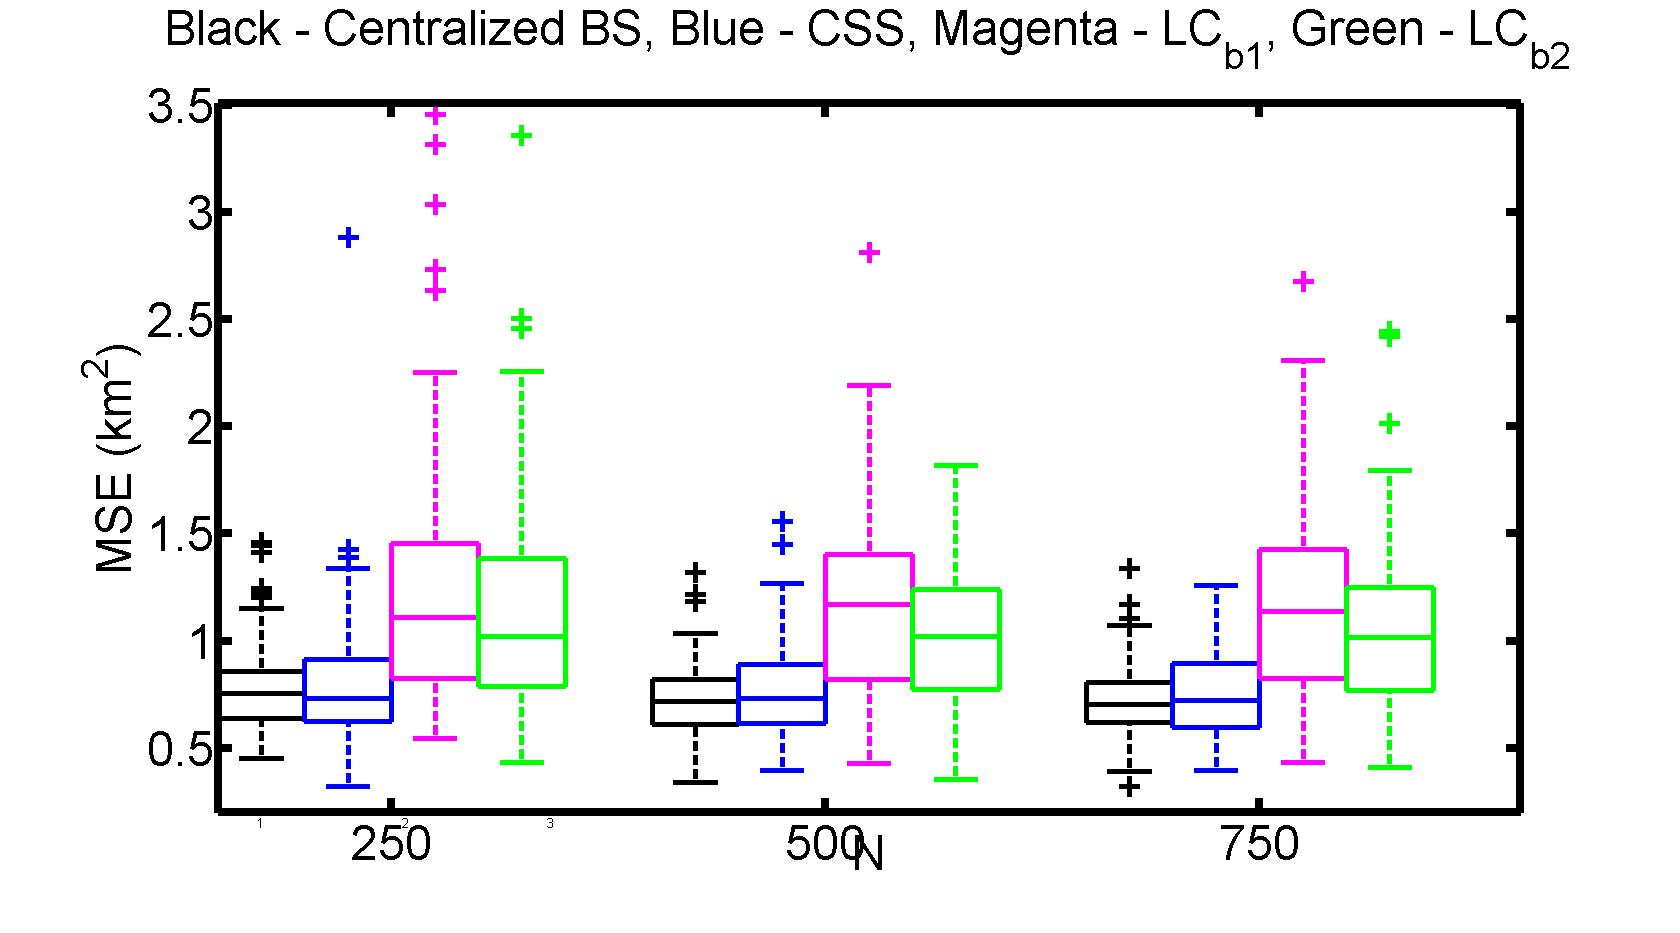
\includegraphics[width=0.75\textwidth]{Figures/MSE}
\caption{Mean squared position error with respect to number of particles}
\label{fig:MSE}
\end{figure}

The BSPF and CSSPF have similar tracking performance; however the LCPF has consistently the worst performance (i.e., almost double the MSE of the other methods). 

%To understand the poor performance of LCPF, at each time step of BSPF, we compute the particle likelihoods exactly and using likelihood consensus approximation, and then compute the discrepancy between them. Fig.~\ref{} shows the average discrepancy over time. 

\section{Conclusion}

\end{document}